\chapter{Research Design and Methods}

\section{Research design}

%What kind of research is this? (e.g. exploratory, confirmatory, intervention-based, evaluationbased, design-based, etc.). Justify the type of research design(s) you intend to use :descriptive (e.g., case study) ;correlational (longitudinal) ; (quasi-)experimental; review etc.

Research questions \ref{benefit}\ref{effectiveness}, \ref{efficiency}, \ref{perception}\ref{usefulness} and \ref{ease} will be investigated using intervention-based research. Because of the systems being used for self-study by the students, they can be individually assigned to a condition, and this enables the use of a true experimental design. Since this will provide the most valid and reliable results, this research design is implemented in this experiment.

Furthermore, research question~\ref{howused} is a qualitative research question, and therefore an interview will take place after the experiment in order to investigate how the students used the system. Next to the interviews, user data and actions will be logged by the server.

The quantitative and qualitative results will be mixed for the purposes of triangulation and expansion as described by \citeA{mixedmethods}. The interviews could provide evidence for the systems being used the intended way. Furthermore, by evaluating how the systems were used insight can be gained into why students had certain perceptions on using the systems. Both triangulation and expansion will be on a partial level of mixing, will take place concurrently, and the quantitative data will be dominant, since the qualitative data exists only to triangulate and expand the quantitative data. Expansion will be added within the research question and integrated within the conclusions whereas triangulation will be added within measurement and integrated within the results. 

\section{Respondents}

%This section is where you describe the who will be approached to participate in your study and how many. Explain how they will be selected (sampling method). Make sure this justification fits your research design and questions.

%1.5.4

More than 100 tenth grade Dutch high school students from the Stedelijk Lyceum in Enschede will be asked to participate in the research. They are concurrent with the experiment, enrolled in a course about 17th century Dutch literature. For this course they already have to prepare themselves for an exam and thereby have incentive to rote memorise the content of the course. To increase the response rate and thereby reduce sampling bias, the students will be rewarded with a bonus point on the exam for participation. In alignment with true experimental design the participant will be assigned to either the flashcard or the flashmap system at random.

\section{Instrumentation}

%Describe the instruments you will use; make a link between the research variables and the instruments explicit (operationalization process) and describe their measurement level if applicable. If you are using existing instruments, provide references.

%n1.5.6

The learning gain will be measured by the means of a pre- and post-test. Both tests will consist of random items from an item bank measuring both knowledge and comprehension levels of the students \cite{bloom}. The tests will be directly based on the concept map, and also will be evaluated by the teacher in order to increase its validity. By using an item bank, the tests will be comparable and thereby the learning gain can be determined by subtracting the score on the pre-test from that on the post-test. Finally the controlled learning gain can be calculated by dividing the learning gain by the time spent on the system. The survey will be based on the standardised Technology Acceptance Model questionnaire \citeA{tamq}.

The interviews will be conducted using a topic list \cite{baarda}, including “frequency”, “usefulness”, “ease of use”, “external conditions”, and “attitudes”, also based on the Technology Acceptance Model. The server logs will contain information about the reaction times, the correct responses, the nodes studied, the time investment, the IP address, and the client, which will be registered per user and per session.

\section{Procedure}

%Describe the procedure for your data collection; what will respondents in your study do? Here you can also address any constraints you may need to cope with in the research and the actions to guard its quality and validity. Potential ethical concerns can be addressed here too.

%n1.6

An outline of the procedure is given in figure~\ref{fig:procedure}.

Before the experiment takes place the experiment will have to be approved by the ethics committee from the University of Twente. After this approval, the students and their parents will be briefed by means of a letter, which consists out of a general description, conditions (voluntary participation and withdrawal at all times), and rewards. They will also both be asked to fill in an informed consent form.

After that, the students with consent will be provided with a general introduction on flashcards by both the teacher and the researcher within the classroom. Then, when the students log into the system for the first time, the server assigns them randomly to either the flashcard or the flashmap condition. By making the introduction ambiguous enough, the students will not be able to recognise this condition in order to guarantee a double-blind experiment.

Before they start using the system they will be asked for general descriptive information such as date of birth and gender. They will not be asked for their names in order to ensure an anonymous identity. Instead a code will be assigned to them making it only able for the teacher to determine the identity. After that the pre-test follows. Then for the next week the students are asked to use the system daily for fifteen minutes. Finally the post-test and survey will be conducted. If the student has used the system for 6 out of 7 days and has filled in the pre- and post-test, they will be awarded with a voucher of \euro{} 5. The system will output a list of student codes of those who should be rewarded. At the end of the post-test, the students can also indicate whether they are willing to participate in the interview.

\begin{figure}
    \centering
    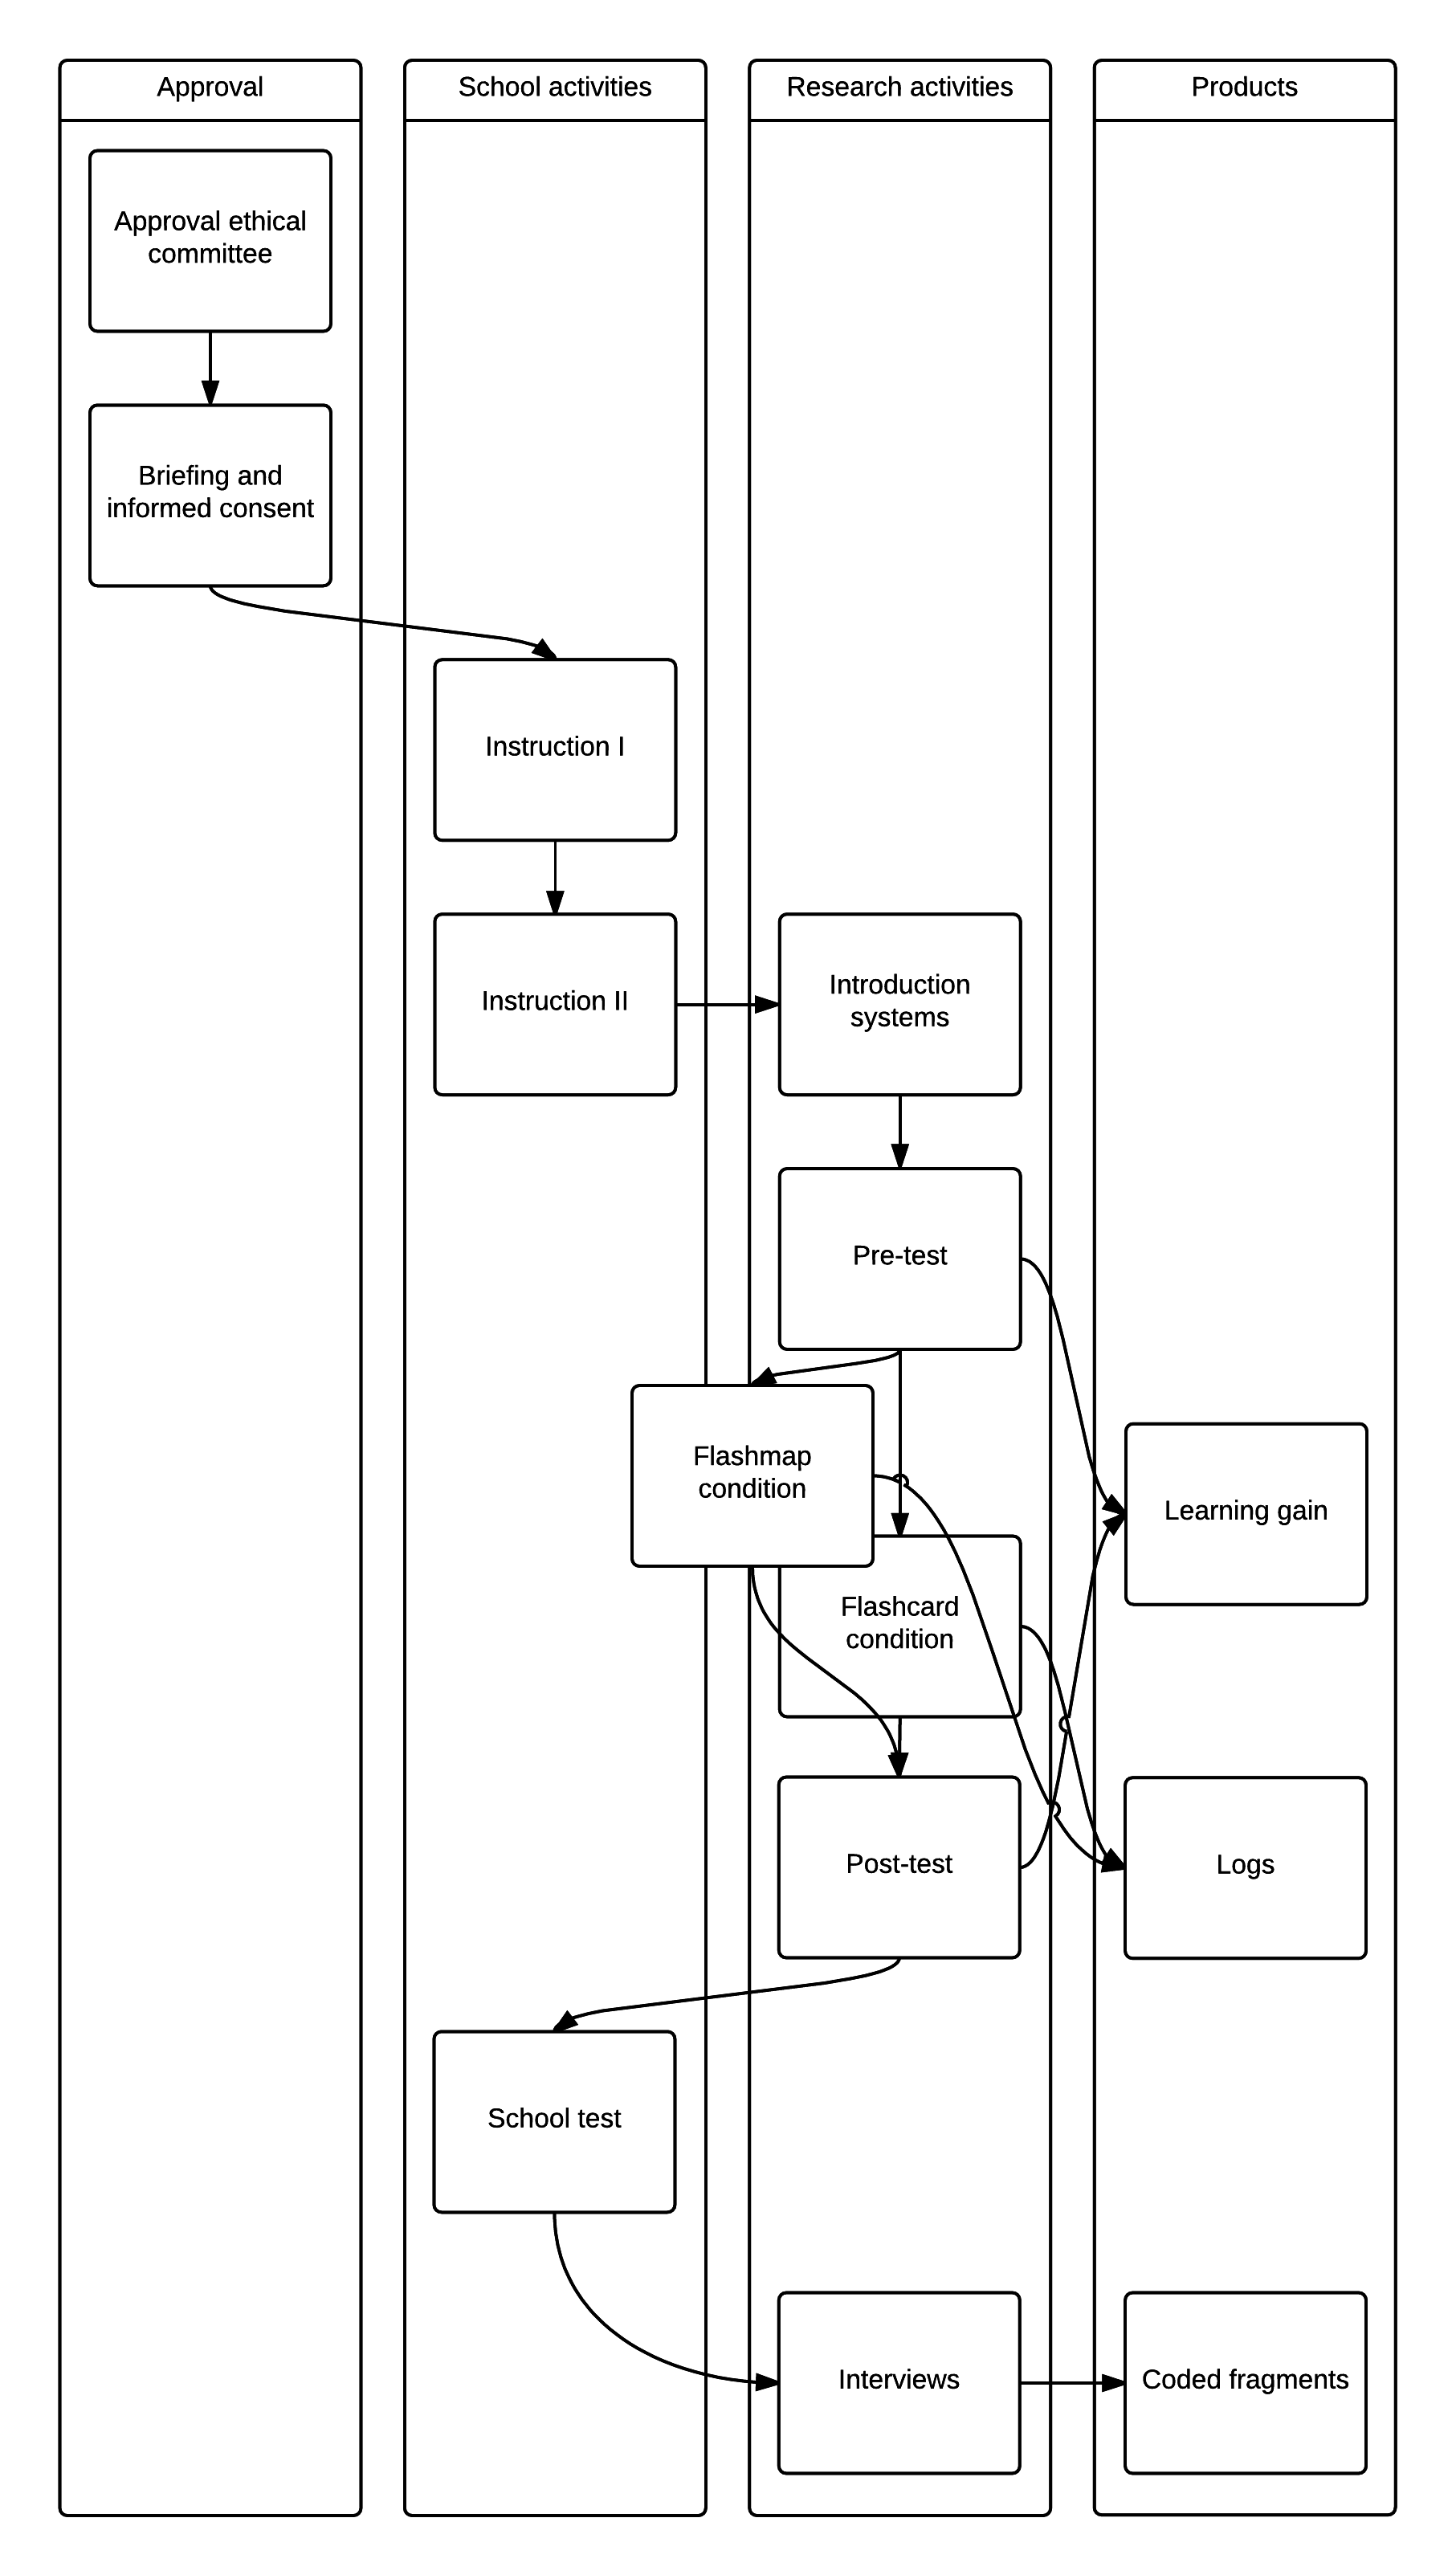
\includegraphics[height=.85\textheight]{img/procedure}
    \caption{An overview of the different steps conducted within the research procedure}
    \label{fig:procedure}
\end{figure}

\section{Data Analysis}

%Describe the type of data you will generate (qualitative, quantitative, mixed-method) and the methods you intend to use to analyze your data. Make sure this fits with your research design and questions. Here you may also address reliability checks for your instrumentation.

Research questions~\ref{benefit}\ref{effectiveness}, \ref{efficiency}, \ref{perception}\ref{usefulness}, and \ref{ease} will be assessed by means of a t-test, using the following hypotheses: 

\begin{tabular}{l l l}
\ref{benefit}\ref{effectiveness} & H0: & $LG_{fc} \leq LG_{fm}$ \\
                                 & Ha: & $LG_{fc} < LG_{fm}$ \\
\ref{benefit}\ref{efficiency}    & H0: & $LGC(fg) \leq LG_{fm}$ \\
                                 & Ha: & $ LGC_{fc} < LG_{fm}$ \\
\ref{perception}\ref{usefulness} & H0: & $U_{fc} \leq U_{fm}$ \\
                                 & Ha: & $U_{fc} < U_{fm}$ \\
\ref{perception}\ref{ease}       & H0: & $E_{fc} \leq E_{fm}$ \\
                                 & Ha: & $E_{fc} < E_{fm}$ \\
\end{tabular}

\noindent where LG = learning gain, LGC = controlled learning gain, U = perceived usefulness, E = perceived ease of use, fc = flashcard condition and fm = flashmap condition. For determining the learning gain, the pre- and post-test have to be scored with a predetermined rubric. The answers will be scored without the scorer being aware whether the question was asked within the pre- or the post-test, or which participant filled in the answer. After both the teacher and the researcher have scored a sample of the answers, the interrater reliability will be calculated. The rest of the answers will be scored by the researcher only, and after scoring all of the items the reliability of test items will be assessed further using Item Response Theory \cite{irt}.

The interviews will be transcribed and coded according to \citeA{baarda}, and another interrater reliability will be determined by a sample of the interviews coded by the researcher and a peer researcher. The coded fragments will be checked to validate the results from the t-tests, together with the server logs made during the experiment.

